\documentclass[aspectratio=169, hyperref={colorlinks=true}]{beamer}
\usepackage[beamer, collink]{prettytex/base}
\usepackage{prettytex/math}
\usepackage{prettytex/gfx}
\usepackage{csquotes}
\usepackage[backend=biber, style=numeric, maxbibnames=20]{biblatex}
% \usepackage[acronym, style=long3col, indexonlyfirst=true, nogroupskip=true]{glossaries}
\usetheme[serif, sansserifheader]{tugrazivc}

\usepackage{xfrac}
\usepackage{dsfont}

\usefonttheme{default}
\addtobeamertemplate{frametitle}{}{\vspace*{-1.5em}}
% \captionsetup{font=small,labelfont=bf}

\definecolor{TUGraz}{HTML}{f70146}
% \definecolor{TUGraz}{HTML}{e4154b}
\definecolor{Accent}{RGB}{136, 58, 234}
\definecolor{AccentGreen}{RGB}{0, 128, 0}
\definecolor{AccentBlue}{RGB}{0, 0, 255}

% \makeglossaries
% \newacronym[shortplural=IAIs, longplural=interpretable artifical intelligence]{iai}{IAI}{interpretable artificial intelligence}


\addbibresource{../../literature/sources.bib}

\title[IVC Seminar SS2025]{In-Silico Cancer Cell}
\author[Peter Waldert]{\textbf{Peter Waldert}}
\date{\today}
\institute{IVC}
\instituteurl{ivc.tugraz.at}

\begin{document}
  \begin{frame}[plain]
    \maketitle
  \end{frame}

  \begin{frame}{The Biological Setting: A Lung-Cancer Cell}
    %% A549 model (lung cancer)
    %% with picture
    \begin{columns}
      \begin{column}{0.42\textwidth}
        \vspace*{-0.4cm}
        \begin{figure}
          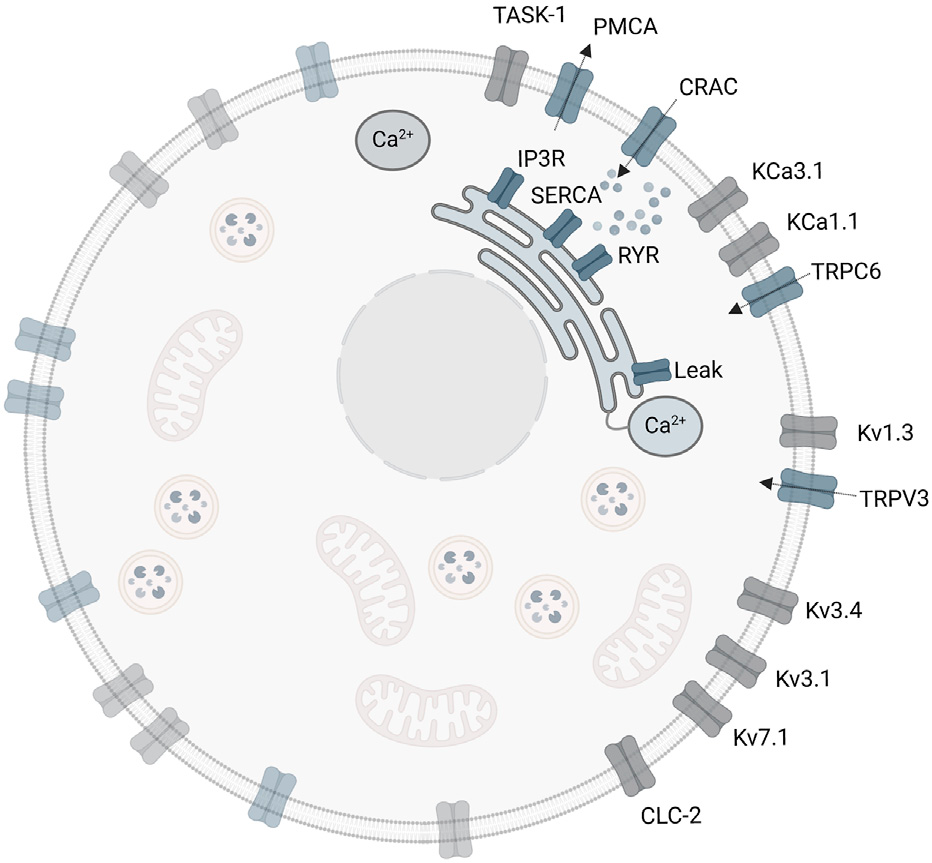
\includegraphics[width=0.9\textwidth]{../../figures/cell-by-langthaler-et-al.png}
          \caption{A549 Cancer Cell Model \cite{2021-A549-model}}
        \end{figure}
      \end{column}
      \begin{column}{0.58\textwidth}
        \begin{itemize}
          \item A human cell is complex. In this project, we focus on the electrophysiological behaviour! \pause
          \item Specifically, on the ion channels on the membrane of an A549 cancer cell. \pause
          \item We improve simulation of the world's first electrophysiological cancer cell model \cite{2021-A549-model}.
          \item And visualise!
        \end{itemize}
      \end{column}
    \end{columns}
  \end{frame}

  \begin{frame}{Experiment: Patch-Clamping}
    %% describe, with picture
    %% we measure current based on voltage changes
    \begin{columns}
      \begin{column}{0.4\textwidth}
        \begin{figure}
          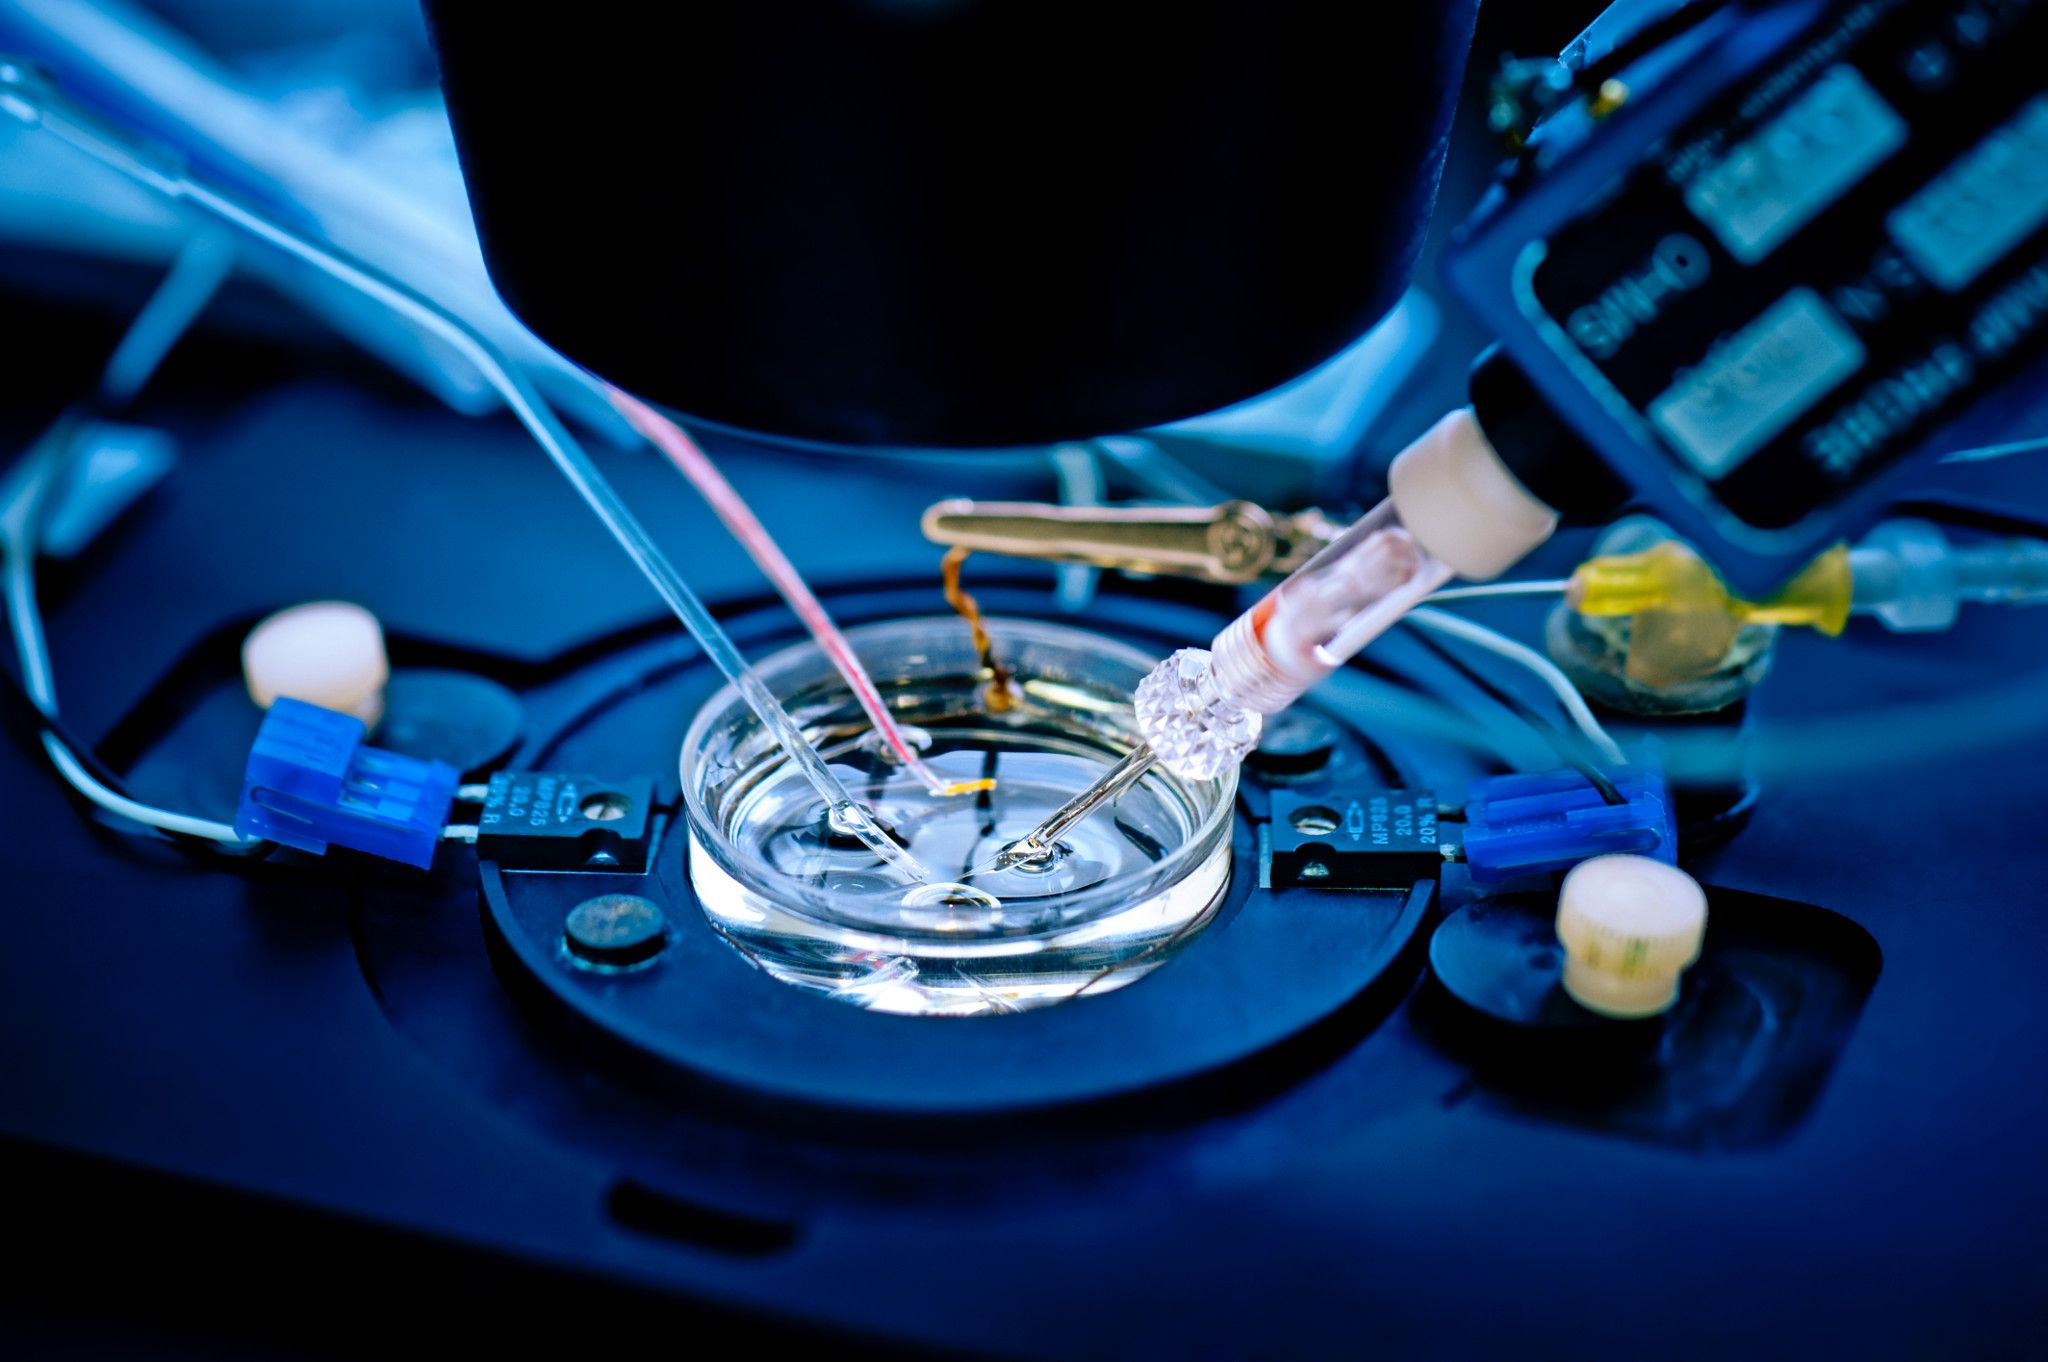
\includegraphics[width=\textwidth]{../../figures/patch-clamp-system.jpeg}
          \caption{Patch-Clamp System \cite{2025-patch-clamp-image}}
        \end{figure}
      \end{column}
      \begin{column}{0.58\textwidth}
        \begin{itemize}
          \item Approach in which electrophysiological behaviour of a cell can be measured in a lab (our data from TU Graz!).
          \item Patch-Clamping can be differentiated into two approaches:
                \begin{itemize}
                  \item the Cell-attached recording method,
                  \item the \emph{Whole-cell recording method}.
                \end{itemize}
        \end{itemize}
      \end{column}
    \end{columns}
  \end{frame}

  \begin{frame}{Simulation of the Experiment}
    %% Multiple independent Ion Channels
    %% Each follows: $$
    \begin{itemize}
      \item We simulate each of the ion channels individually, once per type.
      \item We know the ion channel types from previous research.
      \item Models for each of them have been identified in long-standing collaborative effort.
      \item We combine the models from literature into a full Rust implementation of each.
    \end{itemize}
  \end{frame}

  \begin{frame}{Hidden Markov Model}
    %% very nice, describe transition matrix and dependence on V, t
    The whole cell current $I: T \to \R$ over time $t \in T \subset \R^+$ is the sum of all individual channel contributions $I_k, k \in \{1, ..., M\}$ over $M \in \N$ channel types
    \begin{equation*}
      I(t) := \sum_{k=1}^{M} N_k I_k(t) = \sum_{k=1}^{M} N_k g_k p_{o,k} \left(V(t)-E_k\right)\,.
      \label{eq:current}
    \end{equation*}
    % where $N_k$ is the number of channels of type $k \in \{1, ..., M\}$, $g_k$ is the respective ion channel's conductivity, $p_{o, k} \in [0, 1]$ is the probability of observing the channel in a state where an ion current can flow (``open states''), $V: T \to \R$ is the voltage across the membrane and $E_k \in \R$ the reversal potential.

    At each time step, the next state $\vec{s}_{k,n+1} \in [0, 1]^{N_{s,k}}$ of the $k$-th channel type is obtained by
    \begin{equation*}
      \vec{s}_{k,n+1} = H_{k}\left(V(t_n), \vec{C}(t_n), t_n\right) \vec{s}_{k,n}\,,
      \quad\text{with}\quad
      t_n := \sum_{i=0}^n (\Delta t)_i\,.
    \end{equation*}
    % where $\vec{s}_{k,n} \in [0, 1]^{N_{s,k}}$ is the state vector of ion channel type $k$ at the $n$-th time step, $H_{k}\left(V, \vec{C}, t_n\right) \in [0, 1]^{N_{s,k} \times N_{s,k}}$ the transition matrix for type $k$ with $\sum_{j=1}^{N_{s,k}} \{H_k\}_{i,j} = 1 \;\forall\,i$, $V(t_n)$ the voltage across the membrane at time $t_n$ and $\vec{C}(t_n) \in \R^4$ the concentrations of Kalium, Calcium, Sodium and Chlorine at time $t_n$.
  \end{frame}

  \begin{frame}{Solution of the Inverse Problem}
    \begin{itemize}
      \item We want to find the best possible match between simulation and measurement current, so we take
            $$\vec{N}_{\rm opt} = \argmin_{\vec{N} \in \N_0^M} \int_T \norm{I_{{\rm sim}, \vec{N}}(t) - I_{\rm meas}(t)}^2 \idd t\,,$$
      \item Where we optimise over the set $\N_0^M$ (for $M$ different channel types).
      \item Using some algebra, one can separate the individual models and simulate their current profiles individually.
      \item This makes the problem soluble much more efficiently (see later).
    \end{itemize}
  \end{frame}

  \begin{frame}{Runtime Optimisation}
    The original MatLab implementation ran the entire night, so:
    \begin{itemize}
      \item Improve what we simulate
      \item Improve how we simulate
      \item Improve the inverse solution method
      \item Improve the solver
    \end{itemize}
  \end{frame}

  \begin{frame}[allowframebreaks]{Quadratic Problem Formulation}
    %% using different methods, based on LSQ.
    %% reformulation into a quadratic problem
    After simulation of the individual channel currents, we want to find
    \begin{equation*}
      \vec{N}_{\rm opt} = \argmin_{\vec{N} \in \N_0^M} \frac{1}{2} \norm{R \vec{N} - \vec{d}}^2\,,
      \label{eq:minimization}
    \end{equation*}
    the number of channels per type, with $\vec{d} \in \R^{N_t}$ the experimentally measured current and $R \in \R^{N_t \times M}$ the matrix of all currents $I_k$ per channel type.
    We find
    $$\vec{N}_{\rm opt} \approx \argmin_{\vec{x} \in \R_+^M} f(\vec{x}) = \argmin_{\vec{x} \in \R_+^M} \sfrac{1}{2} \norm{R \vec{x} - \vec{d}}^2\,.$$

    We manipulate the cost function $f: \R^M \to \R^+$,
    \begin{align*}
      f(\vec{x}) & = \sfrac{1}{2} (R \vec{x} - \vec{d})^T (R \vec{x} - \vec{d})                                                          \\
                 & = \sfrac{1}{2} \left(\vec{x}^T R^T R \vec{x} - \vec{x}^T R^T \vec{d} - \vec{d}^T R \vec{x} + \vec{d}^T \vec{d}\right) \\
                 & = \sfrac{1}{2} \left(\vec{x}^T P \vec{x} + \vec{x}^T \vec{q} + \vec{q}^T \vec{x}\right) + \mathcal{O}(1)              \\
                 & = \sfrac{1}{2} \vec{x}^T P \vec{x} + \vec{q}^T \vec{x} + \mathcal{O}(1)
    \end{align*}
    where we let $P := R^T R \in \R^{M \times M}$ and $\vec{q} := -R^T \vec{d} \in \R^M$ and leave out the constant $\vec{d}^T \vec{d}$ as $\mathcal{O}(1)$.

    We can express the nonnegativity constraint $\vec{x} \ge \vec{0}$ as an equality constraint using a slack variable $\vec{s} \in \R_+^M$,
    $$-\vec{x} + \vec{s} = \vec{0} \quad\Leftrightarrow\quad A \vec{x} + \vec{s} = \vec{b}\,\quad \text{with}\quad A = -\mathds{1} \in \R^{M \times M} \;\;\text{and}\;\; \vec{b} = \vec{0} \in \R^M\,.$$
    This leaves us with a constrained \textit{quadratic program},
    \begin{align*}
      \min_{\vec{x} \in \R^M}\; & \sfrac{1}{2}\, \vec{x}^T P \vec{x} + \vec{q}^T \vec{x},  \\
      s.t.\;                    & A \vec{x} + \vec{s} = \vec{b}\,,\; \vec{s} \in \R_+^M\,.
    \end{align*}

    % We solve the quadratic problem in this exact form using Clarabel \cite{2024-clarabel}.
    % Note that in Clarabel notation, the slack variable is to be taken as an element of the nonnegativity cone.

    The integer solution can then be obtained from rounding,
    $$\vec{N}_{\rm opt} = \lfloor \vec{x} \rceil \in \N_0^M\,.$$

    One obtains:
    $$\vec{N}_{\rm opt} = [13, 247, 10, 1176, 38, 7, 24, 188, 15, 10, 234]\,,$$
    for the G0 cell cycle phase.
  \end{frame}

  \begin{frame}{Adaptive Timestepping}
    In order to accelerate the simulation in areas where there is little change to the dynamics, we choose an adaptive step size $(\Delta t)_{n}$ based on
    \begin{equation*}
      (\Delta t)_{n+1} = (\Delta t)_{n} \left(\frac{\Delta^{\rm tol}}{\sum_{k=1}^{M} N_k \norm{\vec{s}_{k,n+1} - \vec{s}_{k,n}}}\right)^{1/2}\,,
      \label{eq:dt-heuristic}
    \end{equation*}
    where the heuristic we choose to stay fast while preventing instability of the simulation, is based on the difference in state change (and also dependent on the channel counts $\vec{N} \in \N_0^M$).
  \end{frame}

  \begin{frame}{Runtime Optimisation}
    %% using adaptive timestepping
    \begin{figure}
      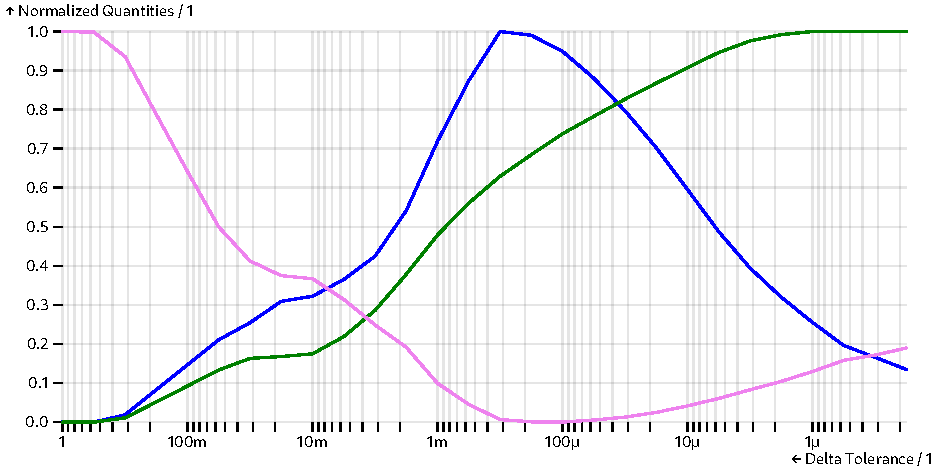
\includegraphics[width=0.65\textwidth]{../../figures/results/delta-tolerance.pdf}
      \caption{
        Relative change of the average timestep $\Delta t$ (in \col{AccentBlue}{blue}), simulation runtime (in \col{Accent}{violet}) and step acceptance rate (in \col{AccentGreen}{green}) when varying the delta tolerance $\Delta^{\rm tol}$.
      }
    \end{figure}
  \end{frame}

  \begin{frame}{Optimisation Approaches}
    % The different approaches were evaluated on the G0 cell cycle phase with the activation voltage protocol. Runtime estimates were obtained on an Intel\texttrademark i7-5600U CPU.
    % \vspace{.5cm}
    \scriptsize
    \begin{table}
      \begin{tabular}{lcrr}
        \hline
        \textbf{Algorithm}                          & \textbf{Abbreviation} & \textbf{Runtime} / ms & \textbf{RMSE} / pA \\
        \hline
        Particle Swarm Optimization                 & PSO                   & 22571                 & 27.69              \\
        Gradient Descent + More Thuente             & GD                    & 18924                 & 32.34              \\
        Limited-Memory BFGS + Hager Zhang           & LBFGS                 & 4845                  & 32.20              \\
        Non-Negative Least Squares \cite{1997-nnls} & NNLS                  & 318                   & 28.00              \\
        Quadratic Program                           & QP                    & 18                    & 28.13              \\
        \hline
      \end{tabular}
      \caption{Comparison of different algorithms for the solution of the inverse problem.}
    \end{table}
  \end{frame}

  \begin{frame}{Visualisation Idea and Accessibility}
    \begin{itemize}
      \item A complicated setup, hard to understand for non-experts
      \item Make the simulation accessible by providing it in multiple formats
      \item Rust linked library, Python (pip) package and visualisation dashboard! \\
            \texttt{pip install in-silico-cancer-cell}
    \end{itemize}
  \end{frame}

  \begin{frame}{Visualisation Dashboard}
    %% Based on Astro and @observablehq/plot, but mostly:
    \begin{figure}
      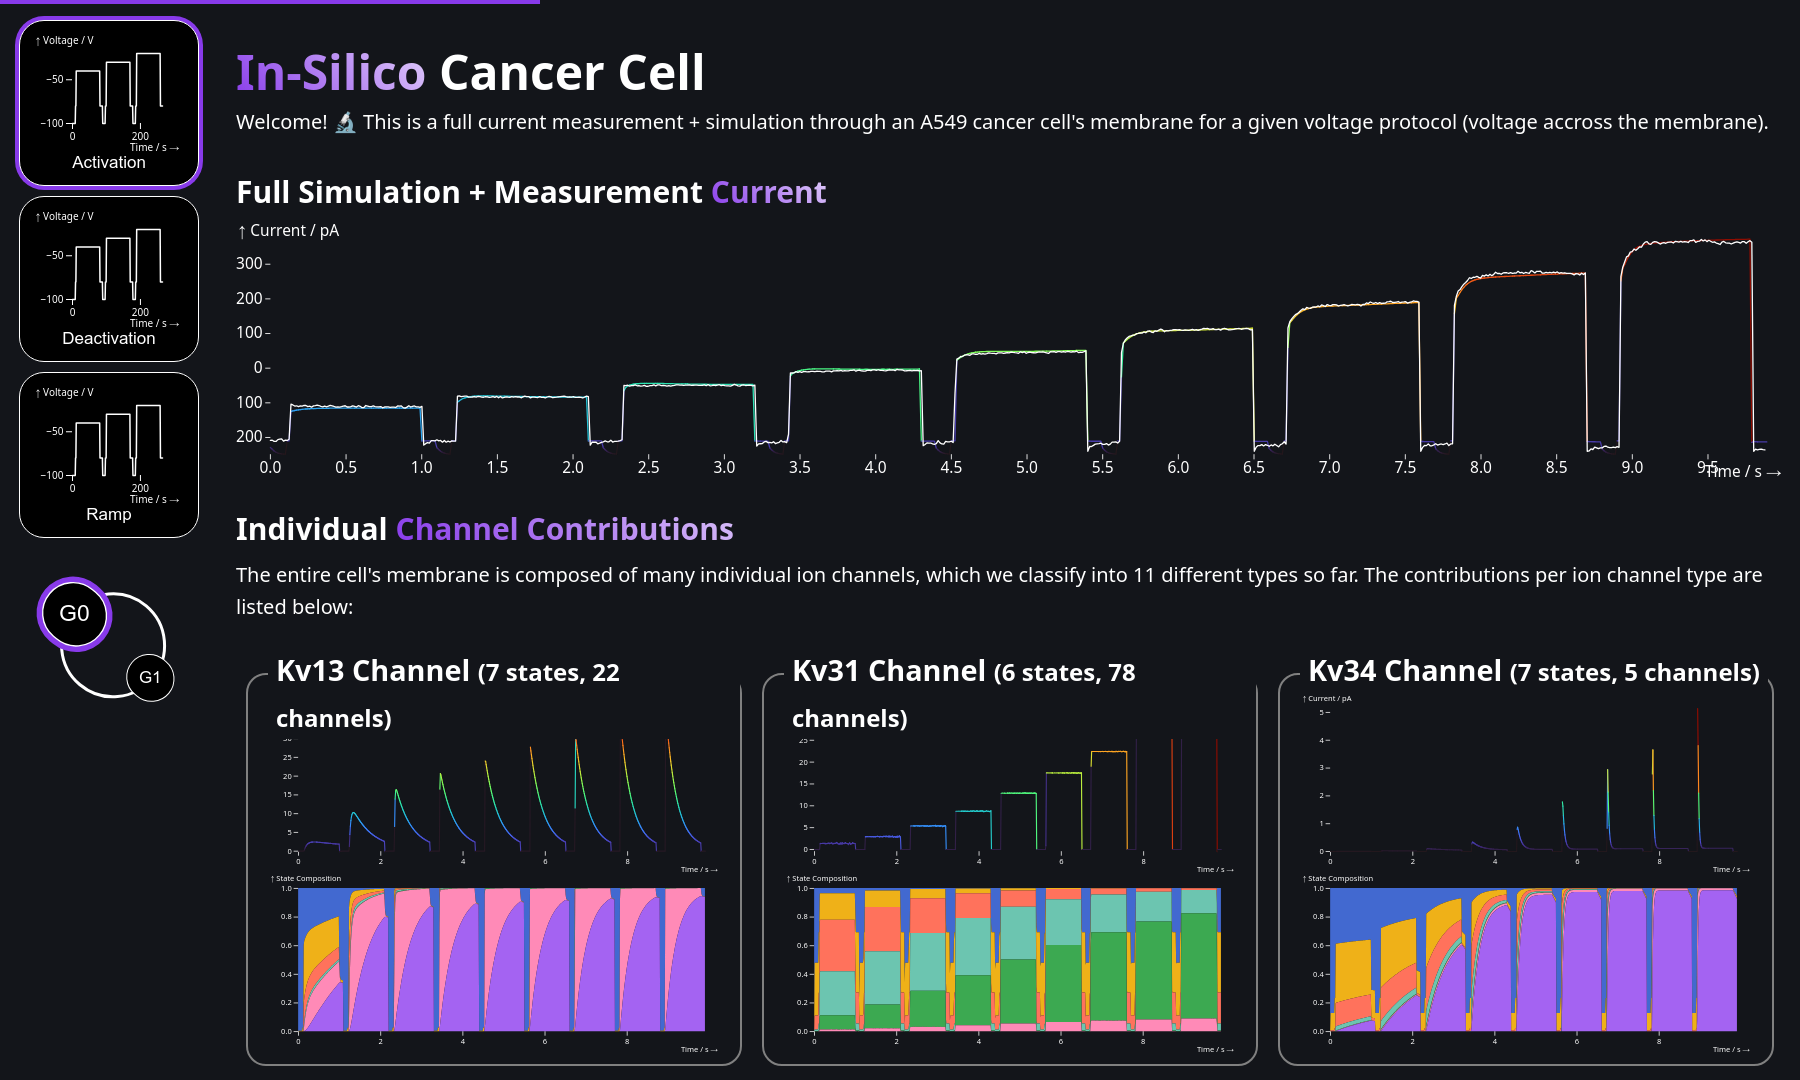
\includegraphics[width=0.7\linewidth]{../../figures/above-the-fold-screenshot.png}
    \end{figure}
  \end{frame}

  \begin{frame}{Compilation to WebAssembly}
    \begin{itemize}
      \item Rust's compiler can target \texttt{wasm} architectures.
      \item Not all functionality is supported in a \texttt{wasm} environment, such as timing.
      \item But of course, numerical code does run and we leverage the compile-time optimisations.
      \item Communicate the results in-memory and visualise them using frontend libraries.
    \end{itemize}
  \end{frame}

  \begin{frame}[allowframebreaks]{References}
    \printbibliography
  \end{frame}
\end{document}
